\documentclass[10pt,landscape,a4paper]{article}
\usepackage[utf8]{inputenc}
\usepackage[ngerman]{babel}
\usepackage[T1]{fontenc}
%\usepackage[LY1,T1]{fontenc}
%\usepackage{frutigernext}
%\usepackage[lf,minionint]{MinionPro}
\usepackage{tikz}
\usetikzlibrary{shapes,positioning,arrows,fit,calc,graphs,graphs.standard}
\usepackage[nosf]{kpfonts}
\usepackage[t1]{sourcesanspro}
\usepackage{multicol}
\usepackage{wrapfig}
\usepackage[top=5mm,bottom=5mm,left=5mm,right=5mm]{geometry}
\usepackage[framemethod=tikz]{mdframed}
\usepackage{microtype}
\usepackage{pdfpages}
\usepackage{amsmath}
\DeclareMathOperator*{\argmax}{\arg\!\max}
\DeclareMathOperator*{\argmin}{\arg\!\min}


\let\bar\overline

\definecolor{myblue}{cmyk}{1,.72,0,.38}

\def\firstcircle{(0,0) circle (1.5cm)}
\def\secondcircle{(0:2cm) circle (1.5cm)}

\colorlet{circle edge}{myblue}
\colorlet{circle area}{myblue!5}

\tikzset{filled/.style={fill=circle area, draw=circle edge, thick},
    outline/.style={draw=circle edge, thick}}
    
\pgfdeclarelayer{background}
\pgfsetlayers{background,main}

\everymath\expandafter{\the\everymath \color{myblue}}
\everydisplay\expandafter{\the\everydisplay \color{myblue}}

\renewcommand{\baselinestretch}{.8}
\pagestyle{empty}

\global\mdfdefinestyle{header}{%
linecolor=gray,linewidth=1pt,%
leftmargin=0mm,rightmargin=0mm,skipbelow=0mm,skipabove=0mm,
}

\newcommand{\header}{
\begin{mdframed}[style=header]
\footnotesize
\sffamily
CZ4041 - Machine Learning
% von~Tim~S.,~Seite~\thepage~von~2
\end{mdframed}
}

\makeatletter % Author: https://tex.stackexchange.com/questions/218587/how-to-set-one-header-for-each-page-using-multicols
\renewcommand{\section}{\@startsection{section}{1}{0mm}%
                                {.2ex}%
                                {.2ex}%x
                                {\color{myblue}\sffamily\small\bfseries}}
\renewcommand{\subsection}{\@startsection{subsection}{1}{0mm}%
                                {.2ex}%
                                {.2ex}%x
                                {\sffamily\bfseries}}



\def\multi@column@out{%
   \ifnum\outputpenalty <-\@M
   \speci@ls \else
   \ifvoid\colbreak@box\else
     \mult@info\@ne{Re-adding forced
               break(s) for splitting}%
     \setbox\@cclv\vbox{%
        \unvbox\colbreak@box
        \penalty-\@Mv\unvbox\@cclv}%
   \fi
   \splittopskip\topskip
   \splitmaxdepth\maxdepth
   \dimen@\@colroom
   \divide\skip\footins\col@number
   \ifvoid\footins \else
      \leave@mult@footins
   \fi
   \let\ifshr@kingsaved\ifshr@king
   \ifvbox \@kludgeins
     \advance \dimen@ -\ht\@kludgeins
     \ifdim \wd\@kludgeins>\z@
        \shr@nkingtrue
     \fi
   \fi
   \process@cols\mult@gfirstbox{%
%%%%% START CHANGE
\ifnum\count@=\numexpr\mult@rightbox+2\relax
          \setbox\count@\vsplit\@cclv to \dimexpr \dimen@-1cm\relax
\setbox\count@\vbox to \dimen@{\vbox to 1cm{\header}\unvbox\count@\vss}%
\else
      \setbox\count@\vsplit\@cclv to \dimen@
\fi
%%%%% END CHANGE
            \set@keptmarks
            \setbox\count@
                 \vbox to\dimen@
                  {\unvbox\count@
                   \remove@discardable@items
                   \ifshr@nking\vfill\fi}%
           }%
   \setbox\mult@rightbox
       \vsplit\@cclv to\dimen@
   \set@keptmarks
   \setbox\mult@rightbox\vbox to\dimen@
          {\unvbox\mult@rightbox
           \remove@discardable@items
           \ifshr@nking\vfill\fi}%
   \let\ifshr@king\ifshr@kingsaved
   \ifvoid\@cclv \else
       \unvbox\@cclv
       \ifnum\outputpenalty=\@M
       \else
          \penalty\outputpenalty
       \fi
       \ifvoid\footins\else
         \PackageWarning{multicol}%
          {I moved some lines to
           the next page.\MessageBreak
           Footnotes on page
           \thepage\space might be wrong}%
       \fi
       \ifnum \c@tracingmulticols>\thr@@
                    \hrule\allowbreak \fi
   \fi
   \ifx\@empty\kept@firstmark
      \let\firstmark\kept@topmark
      \let\botmark\kept@topmark
   \else
      \let\firstmark\kept@firstmark
      \let\botmark\kept@botmark
   \fi
   \let\topmark\kept@topmark
   \mult@info\tw@
        {Use kept top mark:\MessageBreak
          \meaning\kept@topmark
         \MessageBreak
         Use kept first mark:\MessageBreak
          \meaning\kept@firstmark
        \MessageBreak
         Use kept bot mark:\MessageBreak
          \meaning\kept@botmark
        \MessageBreak
         Produce first mark:\MessageBreak
          \meaning\firstmark
        \MessageBreak
        Produce bot mark:\MessageBreak
          \meaning\botmark
         \@gobbletwo}%
   \setbox\@cclv\vbox{\unvbox\partial@page
                      \page@sofar}%
   \@makecol\@outputpage
     \global\let\kept@topmark\botmark
     \global\let\kept@firstmark\@empty
     \global\let\kept@botmark\@empty
     \mult@info\tw@
        {(Re)Init top mark:\MessageBreak
         \meaning\kept@topmark
         \@gobbletwo}%
   \global\@colroom\@colht
   \global \@mparbottom \z@
   \process@deferreds
   \@whilesw\if@fcolmade\fi{\@outputpage
      \global\@colroom\@colht
      \process@deferreds}%
   \mult@info\@ne
     {Colroom:\MessageBreak
      \the\@colht\space
              after float space removed
              = \the\@colroom \@gobble}%
    \set@mult@vsize \global
  \fi}

\makeatother
\setlength{\parindent}{0pt}

\begin{document}
%\footnotesize
\small
\setlength{\columnsep}{3pt}
\begin{multicols*}{5}

\section{Bayesian Classifiers}
\subsection*{Probabilities}
\subsection*{Sum Rule}
$P(A) = \sum_B P(A,B)$\\
$P(A) = \sum_B\sum_C P(A,B,C)$\\
\subsection*{Product Rule}
$P(A,B) = P(B|A)\times P(A) = P(A|B)\times P(B)$\\
\subsection*{Bayes Theorem}
\[P(A|B) = \frac{P(A,B)}{P(B)} = \frac{P(B|A)P(A))}{P(B)}\]\\
(Generalised case)\\
\[P(A_1...A_k|B_1...B_p) = \frac{P(B_1...B_p,A_1...A_k)}{P(B_1...B_p)}\]\\
\subsection*{Bayesian Classifiers}
Bayesian classifiers aim to find the mapping $f: \mathbf{x} \Rightarrow y$
for supervised learning in the form of conditional probability $P(y|\mathbf{X})$
via Bayes rule.
\[P(y|\mathbf{X}) = \frac{P(y, \mathbf{X})}{P(\mathbf{X})} = \frac{P(\mathbf{X}|y)P(y)}{P(\mathbf{X})}\]\\
For a classification with C classes, given a data instance $\mathbf{x^*}$:\\
\[y^* = c^* if c^* = \argmax_c P(y=c|\mathbf{x^*})\]\\
Applying Bayes rule,\\
\[P(y=c|\mathbf{x^*}) = \frac{P(\mathbf{x^*}| y=c)P(y=c)}{P(\mathbf{x^*})}\]\\
Therefore,\\
\[y^* = \argmax_c \frac{P(\mathbf{x^*}| y=c)P(y=c)}{P(\mathbf{x^*})}\]\\
\[= \argmax_c P(\mathbf{x^*}| y=c)P(y=c)\]\\

\section{Bayesian Decision Theory}
Incorporating cost of misclassification on top of simple Bayesian Classifiers.
\subsection*{Loss/Cost}
Actions: $a_c$, i.e., predict $y=c$\\
Define $\lambda_{ij}$ as the cost of $a_i$ when optimal action is $a_j$. E.g.:\\
$\lambda_{00} = 0$ (predict correctly)\\
$\lambda_{11} = 0$ (predict correctly)\\
$\lambda_{01} = 10$ misclassify 1 as 0\\
$\lambda_{00} = 1$ misclassify 0 as 1\\
\subsection*{Expected Risk}
Expected risk for taking action $a_i$:\\
\[R(a_i|\mathbf{x}) = \sum^{C-1}_{c=0}\lambda_{ic}P(y=c|\mathbf{x})\]\\
To classify, for all actions, calculate expected risk, then choose the action 
with the minimum risk.
\subsection*{Special Case: 0/1 loss}
\[\lambda_{ij} = \begin{cases}
    0 \text{ if } i = j \\
    1 \text{ if } i \neq j
\end{cases}\]
$\therefore R(a_i|\mathbf{x}) = 1 - P(y=i|\mathbf{x})$\\
In this case,\\
\[\text{Choose } a_i \text{ if } R(a_i|\mathbf{x}) = \min_{a_c}R(a_c|\mathbf{x})\]
Is equivalent to:\\
\[\text{Predict } y = c^* \text{ if } P(y=c^*|\mathbf{x}) = \max_{c}P(y=c|\mathbf{x})\]



\section{Na\"{i}ve Bayes Classifiers}
\subsection*{Independence}
A is \textbf{independent} of B, if:\\
$P(A,B) = P(A|B)\times P(B) = P(A)\times P(B)$\\
$P(A,B) = P(B|A)\times P(A) = P(A)\times P(B)$\\
Or,\\
$P(A|B) = P(A)$\\
$P(B|A) = P(B)$\\
\subsection*{Conditional Independence}
A is \textbf{conditionally independent} of B, given C if:\\
$P(A|B,C) = P(A|C)$\\
\subsection*{Na\"{i}ve Bayes Classifier}
1. Assumption: conditional independence of features given label\\
\[p(\mathbf{x}|y = c) = P(x_1,...,x_d|y=c)\]
\[ = P(x_1|y=c)P(x_2|y=c)...P(x_d|y=c)\]
\[ = \prod^{d}_{i=1}P(x_i|y=c)\]
To classify a test record $\mathbf{x^*}$, compute the posteriors for 
each class:\\
\[p(y=c|\mathbf{x^*}) = \frac{(\prod^{d}_{i=1}P(x_i^*|y=c))P(y=c)}{P(\mathbf{x^*})}\]
Since $P(\mathbf{x^*})$ is constant for each class c, it is sufficient 
to choose the class that maximises the numerator term.
\[y^* = \argmax_c (\prod^{d}_{i=1}P(x_i^*|y=c))P(y=c)\]\\

\subsection*{Estimating Cond Prob (Discrete)}
\[P(x_i = k| y = c) = \frac{|(x_i - k)\wedge (y=c)|}{|y=c|}\]
\subsection*{Estimating Cond Prob (Continuous)}
\[P(x_i|y=c) = \frac{1}{\sqrt{2\pi \sigma^2_{ic}}}e^{-\frac{(x_i-\mu_{ic})^2}{2\sigma^2_{ic}}}\]
Supposing there are $N_c$ instances in class c,\\
Sample mean:
\[\mu_{ic} = \frac{1}{N_c}\sum^{N_c}_{j=1}x_{ij}\]
Sample variance:
\[\sigma^2_{ic} = \frac{1}{N_c-1}\sum^{N_c}_{j=1}(x_{ij}-\mu_{ic})^2\]

\subsection*{Laplace Estimate}
Alternative prob estimation for discrete features.
\[P(x_i = k| y = c) = \frac{|(x_i - k)\wedge (y=c)|+1}{|y=c|+n_i}\]
where $n_i$ is \#distinct values of $x_i$.
In extreme cases with no training data, $P(x_i = k| y = c) = \frac{1}{n_i}$\\

\subsection*{M-estimate}
A more general estimation:
\[P(x_i = k| y = c) = \frac{|(x_i - k)\wedge (y=c)|+m\times \tilde{P}(x_i = k| y = c)}{|y=c|+m}\]
Where $m$ is a hyperparameter and $\tilde{P}(x_i = k| y = c)$ is prior information of ${P}(x_i = k| y = c)$. 
(e.g., domain knowledge)

Extreme case with no training data: $P(x_i = k| y = c) = \tilde{P}(x_i = k| y = c)$
\section{Bayesian Belief Networks}
Suppose all features are \textbf{discrete} 
(if there are continuous and discrete, estimation is much more difficult)\\\\
Two key elements:\\
1. A directed acyclic graph (DAG) encoding dependence relationships between 
a set of variables\\\\
2. A probability table associating each node to immediate parent nodes

\subsection*{DAG: Conditional Independence}
A node in a Bayesian network is conditionally independent of its 
non-descendants, \textbf{if its parents are known}.
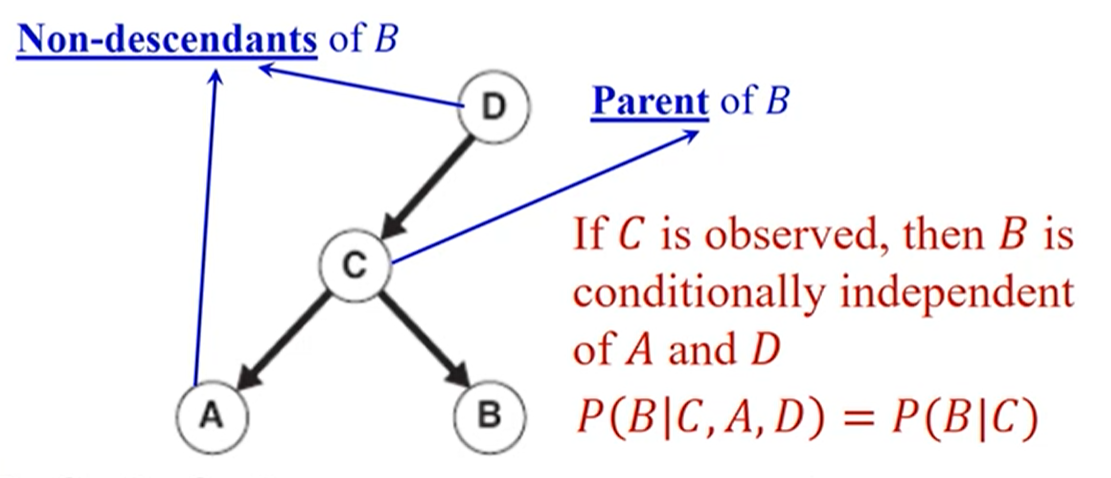
\includegraphics[width=\linewidth]{fig/bbn1}\\\\
\textbf{IMPORTANT!} If A and B are conditionally independent given C, we have:\\
1. $P(A|B,C) = P(A|C)$\\
2. $P(A,B|C) = P(A|C)P(B|C)$
\\

\subsection*{Important! Using BBN for Inference}
Given a BBN, and an inference(prediction) task:\\
1. Translate problem into probabilisitc language\\
2. If the probabilities to be estimated cannot be obtained 
from the probability tables of the BBN, then\\
A. Identify a subgraph which captures the dependence between 
input variables (features) and output variable (class)\\\\
B. Based on the network topology, apply product rule, sum rule
and the properties of conditional independence and independence
to induce equivalent forms of the probabilities until all 
probabilities can be found from the probability tables.
\section{Decision Trees}
- Greedy strategy, split records based on feature test that optimises
certain criterion\\
Key issues:\\
1) How to split the records?\\
- Specifying feature test condition\\
- Determining best split\\
2) When to stop splitting?\\
\subsection*{Determining Test Conditions}
\subsection*{Splitting based on binary features}
2 Possible outcomes (e.g. Yes/No)
\subsection*{Splitting based on discrete features}
- Multi-way split: Use as many partitions as distinct values\\
e.g.: Marital Status $\Rightarrow$ [Single], [Divorced], [Married]
\\\\
- Binary split: Divides possible values as 2 subsets, need to find optimal 
partitioning\\
e.g.: Marital Status $\Rightarrow$ [{Single, Divorced}], [Married]
\subsection*{Splitting based on continuous features}
- Binary split: $(x_j < v)$ or $(x_j \geq v)$\\\\
- Multi-way split (Discretization)\\\\
Consider all possible splits and find the best cut\\
Can be very computationally intensive\\
\subsection*{Determining Best Split}
Using measure of node impurity -- favour split with low degree of impurity
\subsection*{Measure of Impurity: Entropy}
Entropy at a given node t:\\
\[E(t) = -\sum_c P(y=c;t)log_2P(y=c;t)\]
\subsection*{Information Gain}
$\Delta_{info}=E(\text{parent}) - E(\text{children})$
\\
To get entropy for children, get entropy of all children nodes and 
normalize by \# of training examples in each child node. Suppose a parent 
node t is split into P partitions (children),\\
$\Delta_{info}=E(t) - \sum^{P}_{j=1}\frac{n_j}{n}E(j)$\\\\
Disadvantage: Tends to prefer splits that result in large number of partitions.
\subsection*{Penalizing large number of partitions (Gain Ratio)}
\[\Delta_{\text{InfoR}} = \frac{\Delta_{\text{info}}}{\text{SplitINFO}}\]
\[\text{SplitINFO} = -\sum^{P}_{i=1}\frac{n_i}{n}log_2(\frac{n_i}{n})\]
\subsection*{Stopping Criterias}
1. All data belong to same class\\
2. Stop expanding when all data have similar feature vals\\
3. Early termination (avoid overfitting)
\newpage
\section{Generalisation}
\underline{Overfitting}: Test error rate increase when training error decrease\\
\underline{Underfitting}: Model too simple, both training and test error large\\
\\
\underline{Training errors}: error on training set, $e(T)$\\
\underline{Generalisation errors}: error on previously unseen testing set, $e'(T)$\\
\subsection*{Estimating Generalisation Errors}
\subsection*{Optimistic Estimate}
Assume training set is good representation of overall data\\
$e'(T) = e(T)$\\
Decision tree induction algo select model with lowest training error rate.\\
\subsection*{Occam's Razor}
Include information of model complexity when evaluating a model.\\
$e'(T) = e(T) + N\times k$\\
where N is the number of leaf nodes and k is a hyperparameter $k > 0$
\subsection*{Using Validation Set}
Divide training data to 2 subsets, 1 for training and 1 for estimating
generalisation error.

\subsection*{Addressing overfitting}
\subsection*{Pre-Pruning}
- Stop if number of instances is less than user-specified threshold\\
- Stop if expanding current node does not improve generalisation errrors
\subsection*{Post-Pruning}
- Grow tree to its entirety\\
- Trim nodes in bottom-up fashion\\
- If generalisation error improves after trimming, replace sub-tree by new leaf\\
\section{KNN Classifiers}
- Instance based, lazy learner - no model built\\
- - "Training"\ is very efficient\\
- - Classifying unknown test instances are relatively expensive\\
- Requires training data to be stored in memory\\\\
Classification steps:\\
1. Compute distance to other training instances\\
2. Identify K nearest neighbors\\
3. Use class labels of neighbors to determine class of instance\\\\
\subsection*{Choosing K}
- K too small, sensitive to noise\\
- K too large, neighborhood may include points from other classes\\
\subsection*{Distance Metric}
Euclidean distance:\\
\[d(\mathbf{x}_i,\mathbf{x}_j) = \sqrt{\sum^{d}_{k=1}(x_{ik} - x_{jk})^2}\]
\subsection*{Voting Schemes}
- Majority voting (sensitive to choice of k)\\
- Distance-weight voting (weight the influence of neighbor $x_i$ according to distance to test data)\\
\[w_i = \frac{1}{d(x^*, x_i)^2}\]
\[y^* = \argmax_c \sum_{(x_i, y_i)\in\mathcal{N}_{x^*}} w_i \times I(c = y_i) \]
\subsection*{Other issues with KNN}
Scaling issues - features may need to be scaled\\
Solution: Normalisation on features of different scales.
\subsection*{Normalisation}
- Min-max normalisation\\
\[v_{\text{new}} = \frac{v_{\text{old}}-\text{min}_{\text{old}}}{\text{max}_{\text{old}}-\text{min}_{\text{old}}}(\text{max}_{\text{new}}-\text{min}_{\text{new}}) \]
- Standardisation (z-score normalisation)\\
($\mu$: mean, $\sigma$:standard deviation)\\
\[v_{\text{new}} = \frac{v_{\text{old}} - \mu_{\text{old}}}{\sigma_{\text{old}}}\]

\section{ANN}
$y = \text{sign}(\mathbf{w} \cdot \mathbf{x})$\\
$w_0 = -\theta,\ X_0 = 1$\\
Where $\theta$ is the threshold term, $\mathbf{w}$ is the weights vector and 
$\mathbf{x}$ is the input vector. An additional dimension is added to both vectors 
such that the sum of products would minus the threshold term, $\theta$.
\subsection*{Activation functions}
\subsection*{Sign Activation function}
\[\text{sign}(z) = \begin{cases}
    1,\hfill z\geq 0\\
    -1,\hfill \text{otherwise}
\end{cases}\]
Since function is not differentiable, 
when finding derivative of the activation function, we set 
y = z, and the derivative of y with respect to z would be = 1

\subsection*{Sigmoid Activation function}
\[a(z) = \frac{1}{1+e^{-\lambda z}}\]
When $\lambda = 1$, it's called the sigmoid function.\\\\
Derivative of sigmoid: 
\[\frac{\partial \hat{y}(z)}{\partial z} = y(z)\cdot (1 - y(z))\]


\subsection*{Error/Loss}
\[E = \frac{1}{2}(y_i - \hat{y}_i)^2\]
\subsection*{Updating Weights}
\[\mathbf{w}_{t+1} = \mathbf{w}_{t} - \lambda \frac{\partial E(\mathbf{w})}{\partial \mathbf{w}}\]
Applying chain rule:
\[\mathbf{w}_{t+1} = \mathbf{w}_{t} - \lambda \frac{\partial E(\hat{y})}{\partial \hat{y}}\frac{\partial \hat{y}(z)}{\partial z}\frac{\partial z(\mathbf{w})}{\partial \mathbf{w}}\]
\[\mathbf{w}_{t+1} = \mathbf{w}_{t} - \lambda (-(y_i - \hat{y}_i))(1)(\mathbf{x}_i)\]
\[\mathbf{w}_{t+1} = \mathbf{w}_{t} - \lambda (-(y_i - \hat{y}_i))(1)(\mathbf{x}_i)\]
\[\mathbf{w}_{t+1} = \mathbf{w}_{t} + \lambda (y_i - \hat{y}_i)\mathbf{x}_i\]

\section{Support Vector Machines}
\subsection*{Decision Boundary}
The decision boundary of a SVM can be defined as:\\
$w_1x_1 + w_2x_w + b = 0$\\
General form:\\
$\mathbf{w}\cdot\mathbf{x} + b = 0$\\
\subsection*{Making predictions}
During training, the values of $\mathbf{w}$ and $b$ is learned.\\\\
For any test example $\mathbf{x}^*$\\
\[\begin{cases}
    f(\mathbf{x}^*) = +1, \text{if} \mathbf{w}\cdot\mathbf{x}^*+b\geq0\\
    f(\mathbf{x}^*) = -1, \text{if} \mathbf{w}\cdot\mathbf{x}^*+b<0
\end{cases}\]
\subsection*{Other notes (Linear Algebra):}
\textbf{Inner Product}\\
\[\mathbf{u} \cdot \mathbf{v} = \sum^{d}_{i=1}(u_i\times v_i) \]
\[\mathbf{u} \cdot \mathbf{v} = ||\mathbf{u}||_2\times||\mathbf{v}||_2\times cos(\theta) \]

\textbf{L2 Norm (Length of vector)}
\[||\mathbf{u}||_2 = \sqrt{\mathbf{u}\cdot\mathbf{u}} = \sqrt{\sum^{d}_{i=1}(u_i\times u_i)} \]
\subsection*{Induction}
- Direction of $\mathbf{w}$ is orthogonal (perpendicular) to the decision boundary.\\\\
Parallel hyperplanes:\\
$\mathbf{w}\cdot\mathbf{x} + b = k$\\
$\mathbf{w}\cdot\mathbf{x} + b = -k$\\
(After rescaling $\mathbf{w} = \mathbf{w}/k$, $b = b/k$)\\
$\mathbf{w}\cdot\mathbf{x} + b = 1$\\
$\mathbf{w}\cdot\mathbf{x} + b = -1$\\\\
\[||\mathbf{w}||_2 \times d = 2\]
\[d=\frac{2}{||\mathbf{w}||_2}\]
\subsection*{Margin Maximisation}
Therefore, decision boundary can be learnt by maximising the margin, $d=\frac{2}{||\mathbf{w}||_2}$. However, this is not easy.
Change this into a minimisation problem.\\
Minimise: $\frac{||\mathbf{w}||_2^2}{2}$\\
Constraints:\\
$\mathbf{w}\cdot\mathbf{x}_i + b \geq 1, \text{if} y_i = 1$\\
$\mathbf{w}\cdot\mathbf{x}_i + b \leq -1, \text{if} y_i = -1$\\
OR, $y_i \times (\mathbf{w}\cdot\mathbf{x}_i + b) \geq 1$
\subsection*{Optimisation Problem for SVM}
\[min_{w,b} \frac{||\mathbf{w}||_2^2}{2}\]
\[\text{s.t.} y_i \times (\mathbf{w}\cdot\mathbf{x}_i + b) \geq 1\]
\subsection*{Multi-Class SVM}
Given 3-class problem $C_1$, $C_2$ and $C_3$\\
Create 3 SVM binary classifiers:
1. Positive $C_1$, Negative $C_2$ \& $C_3$\\
2. Positive $C_2$, Negative $C_1$ \& $C_3$\\
3. Positive $C_3$, Negative $C_1$ \& $C_2$\\\\
Use majority voting to determine class for test example.
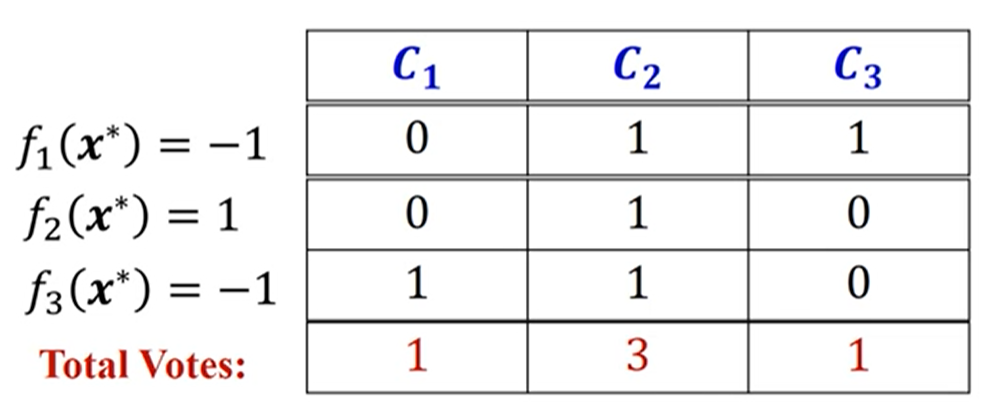
\includegraphics[width=\linewidth]{fig/multiclasssvm.PNG}


\section{Linear Regression}
\subsection*{Error for 1-D Linear Regression Model}
Sum-of-squares (SSE) error:
\[E(w) = \frac{1}{2}\sum^N_{i=1}(w \times x_i - y_i)^2\]

Learn linear model in terms of w by minimising the error\\
\[w^* = \argmin_w E(w)\]
To solve the unconstrained minimisation problem, set derivative of $E(w)$ w.r.t $w$ to zero
\[\frac{\partial E(w)}{\partial w} = \frac{\partial (\frac{1}{2}\sum^N_{i=1}(w \times x_i - y_i)^2)}{\partial w} = 0\]
Closed form solution:
\[w = \frac{\sum^N_{i=1} y_i \times x_i}{\sum^N_{i=1} x_i^2}\]
\subsection*{More general case (multi-dimension)}
$f(\mathbf{x}) = \mathbf{w}\cdot\mathbf{x} + b$\\\\
- By defining $w_0 = b$ and $X_0 = 1$, $w$ and $x$ are of d+1 dimensions\\
$f(\mathbf{x}) = \mathbf{w}\cdot\mathbf{x}$
\subsection*{Error for Linear Regression Model}
\[E(\mathbf{w}) = \frac{1}{2}\sum^N_{i=1}(\mathbf{w} \cdot \mathbf{x}_i - y_i)^2\]
Learn linear model in terms of $\mathbf{w}$ by minimizing the error (with regularisation term)
\[\mathbf{w^*} = \argmin_w E(\mathbf{w}) + \frac{\lambda}{2}||\mathbf{w}||_2^2\]
\subsection*{Closed-Form Solution}
\[\mathbf{w} = (\mathbf{X}^T\mathbf{X} + \lambda \mathbf{I})^{-1}\mathbf{X}^Ty\]
\section{Ensemble Learning}
\subsection*{Necessary Conditions}
1) Base classifiers are independent of each other\\
2) Base classifiers should do better than classifier that performs random guessing (i.e., acc > 0.5)
\subsection*{Error rate of ensemble}
Supposing N independent base classifiers with error $\epsilon$:\\
\[P = \sum^N_{i = (N//2) + 1} \epsilon^i(1-\epsilon)^{N-i}\]
\subsection*{Ensemble Methods}
\subsection*{Bagging}
- Sample examples \textbf{with replacement} and build model on each bootstrap sample.\\
- Use majority voting to determine class label of ensemble classifier\\
- A bootstrap sample contains approximately 63.2\% of original training data
\subsection*{Boosting}
1) Initially, all examples are assigned equal weights\\
2) Bootstrap sample is drawn and a model is trained from sample\\
3) Model is then used to classify examples from training set\\
4) Update weights of examples after the end of boosting round\\
\begin{itemize}
    \item Wrongly classified - increase
    \item Correctly classified - decrease
    \item Examples not drawn - unchanged
\end{itemize}
5) Use weighted voting, each classifier would have different weights
\subsection*{Random Forests}
- Specifically designed for decision tree classifiers
1) Choose T, number of trees to grow\\
2) Choose m', number of features used to calculate best split (Typically 20\%)\\
3) For each tree\\
- Choose training set via bootstrapping\\
- For each node, randomly choose m' features and calculate best split\\
- Trees fully grown and not pruned\\
4) Use majority vote among all trees
\subsection*{Combination Methods}
- Majority voting\\
- Weighted voting\\
- Simple average:\\
$f_M(\mathbf{x}) = \frac{1}{T}\sum^T_{i=1}f_i(\mathbf{X})$\\
- Weighted average:\\
$f_M(\mathbf{x}) = \frac{1}{T}\sum^T_{i=1}w_if_i(\mathbf{X})$\\
Where $w_i \geq 0$, and $\sum^T_{i=1}w_i = 1$\\
\subsection*{Combining by Learning}
Combiner: second-level learner, or meta-learner\\
Combiner takes output of base classifiers as features, and learn to classify 
based on output label.
\section{Clustering}
\subsection*{Cluster Analysis}
- Finding groups of data instances such that data instances in a group are:
\begin{itemize}
    \item Similar to one another
    \item Different from data in other groups
\end{itemize}
It is \textbf{NOT}:\\
- Supervised classification (class label info available)\\
- Simple segmentation (e.g. divide examples into groups by properties/feature value)\\

\subsection*{Types of clusterings}
- Partitional (non-overlapping)\\
- Hierarchical (nested)\\
- Exclusive/Non-exclusive (instance belonging to multiple cluster)\\
- Fuzzy/Non-fuzzy (point belongs to every cluster with weight (sums to 1))\\
- Partial/Complete (Only some instances clustered for partial)\\

\subsection*{K-means}
- Partitional clustering\\
Preprocessing:\\
- Normalize data\\
- Eliminate outliers\\\\
Algorithm:\\
1) Select k data as initial centroids\\
Loop while centoids' values are updated,\\
2) Form k clusters by assigning data instances to closest centroid\\
3) Recompute the centroid of each cluster (mean of data instances in cluster)\\\\
Note: performance affected greatly by choie of initial centroids.

\subsection*{Evaluation of K-means clusters}
Total Sum of squared error (SSE)\\
\[SSE = \sum^K_{i=1}\sum_{\mathbf{x}\in C_i} \text{dist}(\mathbf{c}_i, \mathbf{x})^2\]

\subsection*{Solving Initial Centoids Issue}
1) Multiple runs, choose run with lowest SSE\\
2) Post-processing:\\
- Decompose cluster with high Cluster SSE\\
- Merge clusters with low cluster SSE, which are close to each other\\
3) Bisecting K-means

\subsection*{Empty Clusters Issue}
Choose replacement centroid:\\
- Choose point that contributes most to SSE\\
- Choose a point from cluster with highest cluster SSE\\
- Repeat several times if there are multiple empty clusters\\

\subsection*{Bisecting K-means}
Start with 1 cluster containing all points\\
While the number of clusters is less than K:\\
1) Select the cluster with the largest SSE\\
2) Bisect the cluster with simple K-means (2 cluster) T times,\\
2a) Choose the split with the lowest SSE from the T number of results\\
2b) Add the split clusters into the list of clusters\\

\subsection*{K-means limitations}
K-means has problems when clusters have differing:\\
- Sizes\\
- Densities\\
Or when clusters have non-globular shapes\\
K-means also sensitive when data has outliers

\subsection*{Hierarchical Clustering}
- Nested clusters organised as hierarchical tree\\
(Visualised as dendrogram)\\\\
Strengths:\\
- Do not have to assume number of clusters, can obtain desired 
number by cutting the dendrogram at the proper level.\\\\
Types:\\
- Agglomerative (Start with 1 cluster per instance, then merge until 1 big cluster)\\
- Divisive (Start with 1 cluster with all points, split at each step until 1 cluster/instance or when 
there are K clusters)

\subsection*{Agglomerative}
- Merge most similar clusters at each step\\
- Update cluster proximity based on type of Inter-Cluster Similarity:\\
- MIN: Proximity = closest points in different clusters\\
- MAX: Proximity = furthest points in different clusters\\
- Group Average: Proximity = average of pairwise distance for all points in clusters\\

\subsection*{Limitations}
- Once clusters are combined, can't be undone (errors propogated)\\
- No objective function is minimized\\
- Different schemes have issues with the following:\\
1) Sensitive to noise/outliers\\
2) Difficulty handling different sized clusters\\

\subsection*{Divisive Hierarchical Clustering}
Algorithm:\\
1) Generate minimum spanning tree to collect all instances as single cluster\\
2) While all clusters are not singleton clusters (Or while number of clusters < K):\\
3) Create a new cluster by breaking the link corresponding to largest distance.

\subsection*{Building MST}
Algorithm:\\
1) Start with tree with a single point (random)\\\\
While there are points not in the tree:\\
2) Look for the closest pair of points such that 1 point is in current tree and the other is not.\\
3) Add the point into the tree and an edge (with a value of the distance) between the two points


\section{Density Estimation}
Goal: Estimate unobservable underlying probability density from observed data.\\\\
Note, probability = area under density fn curve. Integrating entire curve gives 1.\\
\subsection*{Approaches for Density Estimation}
- Parametric density estimation\\
- Nonparametric density estimation\\
\subsection*{General Principle}
Observed data points assumed to be sample of N random variables \textbf{independent 
and identically distributed (i.i.d.)}\\
\underline{Identically Distributed}: For any $x_i \in D$, it is sampled from 
sampled from same probability distribution\\
\underline{Independent}: all data points $x_i \in D$ are independent events.

\subsection*{Parametric Density Estimation}
Assume that data are drawn from known probability density family, $p(\mathbf{x}; \theta)$,
defined up to parameters, $\theta$.\\
Task: Find parameter $\theta$ that makes sampling $x_i$ from $p(\mathbf{x}; \theta)$
as likely as possible.\\\\
Approach: \textbf{Maximum Likelihood Estimation}
\subsection*{Maximum Likelihood Estimation}
Likelihood of parameter $\theta$ given sample $\mathcal{D}$: $l(\theta|\mathcal{D}) \triangleq p(\mathcal{D};\theta)$\\
Since data are i.i.d, the likelihood is product of likelihoods of individual data points:\\
\[l(\theta|\mathcal{D}) \triangleq p(\mathcal{D};\theta) = \prod^N_{i=1}p(x_i; \theta)\]
Therefore, find $\theta$ that makes $\mathcal{D}$ most likely to be drawn:
\[\hat{\theta} = \argmax_\theta l(\theta|\mathcal{D})\]
Typically, log-likelihood is used such that product can be converted into sum\\
\[ln\ l(\theta|\mathcal{D}) = \sum^N_{i=1}ln\ p(x_i; \theta)\]
\subsection*{Univariate Gaussian}
\[\mathbf{x}_i \thicksim p(\mathbf{x};\mu, \sigma^2) = \frac{1}{\sqrt{2\pi \sigma^2}}e^{(-\frac{(x-\mu)^2}{2\sigma^2})}\]
Solutions to parameters $\mu$ and $\sigma^2$ (Unbiased estimation):\\
\[\begin{cases}
    \hat{\mu} = \frac{1}{N}\sum^N_{i=1}\mathbf{x}_i \\\\
    \hat{\sigma^2} = \frac{1}{N-1}\sum^N_{i=1}(\mathbf{x}_i - \hat{\mu})^2 
\end{cases}\]
\subsection*{Multivariate Gaussian}
Solutions to parameters $\mu$ (d-dimensional mean vector)\\
and $\Sigma$ (d x d covariance matrix) (Unbiased estimation):\\

\[\begin{cases}
    \hat{\mathbf{\mu}} = \frac{1}{N}\sum^N_{i=1}\mathbf{x}_i \\\\
    \hat{\mathbf{\Sigma}} = \frac{1}{N-1}\sum^N_{i=1}(\mathbf{x}_i - \hat{\mathbf{\mu}})(\mathbf{x}_i - \hat{\mathbf{\mu}})^T
\end{cases}\]

\subsection*{Nonparametric density estimation}
\subsection*{Histogram Estimator}
\[\hat{p}(\mathbf{x})=\frac{\# x_i \text{ in same bin as } x}{N\Delta}\]
First bin start from 0, therefore determine which bin to use by using x
\subsection*{Na\"ive Estimator}
\[\hat{p}(\mathbf{x})=\frac{1}{N\Delta}\sum^N_{i=1}w(\frac{\mathbf{x} - \mathbf{x}_i}{\Delta})\]
Windowing function
\[w(u) = \begin{cases}
    1 \text{ if } -\frac{1}{2} \leq u < \frac{1}{2}\\
    0 \text{ otherwise}
\end{cases}\]

\subsection*{Generalisation to Multivariate}
If the data is d-dimensional, the bins become a d-dimensional hypercube with volume: $V=h^d$, where h is the length of each edge 
and d is the number of dimensions.

Windowing function:\\
\[w(u) = \begin{cases}
    1 \text{ if } -\frac{1}{2} \leq u_j < \frac{1}{2} \text{ for all } j \in \{1,.,d\}\\
    0 \text{ otherwise}
\end{cases}\]
\[\hat{p}(\mathbf{x})=\frac{1}{NV}\sum^N_{i=1}w(\frac{\mathbf{x} - \mathbf{x}_i}{h})\]


\subsection*{KNN Estimator}
Set the numerator as a constant (K), adapt smoothing to 
local density of data. Degree of smoothing controlled by K (number of neighbours).
\[p(\mathbf{x}) = \frac{K}{NV_x}\]
$V_x$ is the volume of the space centered at $\mathbf{x}$ that exactly contains K nearest 
neighbors of $\mathbf{x}$.\\\\

With a predefined K, for a data point $\mathbf{x}$,\\
1) Compute distance of all points to x (e.g. euclidean dist)\\
2) Sort observed data points based on distances in asc order\\
3) Obtain the k-th distance to compute $V_{d_k(\mathbf{x})}$, which is the volume 
of the d-ball\\
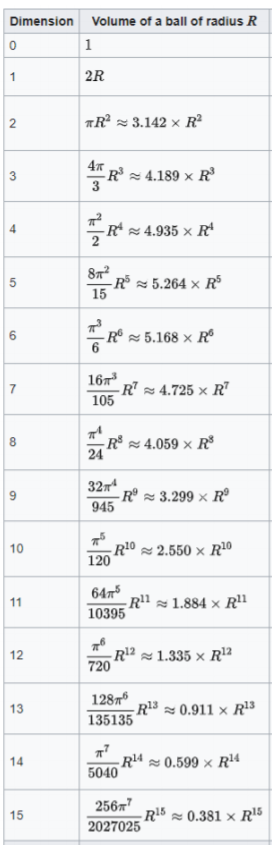
\includegraphics[width=\linewidth]{fig/knnestimator.PNG}

\columnbreak
\section{Dimensionality Reduction}
- Summarise observed high-dimensional data points to low-dimensional vectors\\
- Avoid curse of dimensionality (Distance-based methods suffer with high dim)\\
- Reduce time/mem needed\\
- Allows visualisation (2D/3D)\\
- Reduce noise\\
\subsection*{Approaches}
- Feature selection (select subset of features)\\
(brute-force / greedy search)\\\\
- Feature Extraction\\
\textbf{Learn} k \textbf{new} features from original d features to 
represent each data instance.\\
--Linear combination of original features, e.g. (PCA)
\subsection*{Principal Component Analysis}
Algorithm:\\
1) Centering data points s.t. mean is 0\\
2) Compute sample covariance matrix\\
\[\tilde{\Sigma} = \frac{1}{N-1}\sum^N_{i=1}\mathbf{x}_i\mathbf{x}_i^T\]
Which is equavalent to:
\[\tilde{\Sigma} = \frac{1}{N-1}X^TX\]

3) Compute eigenvectors of $\tilde{\Sigma}$, $\{\mathbf{u}_1,\mathbf{u}_2,...,\mathbf{u}_d\}$
which are sorted based on their eigenvalues in non-increasing order,
i.e., $\lambda_1 \geq \lambda_2 \geq ... \geq \lambda_d$\\
4) Select first k eigenvectors to construct principal components\\
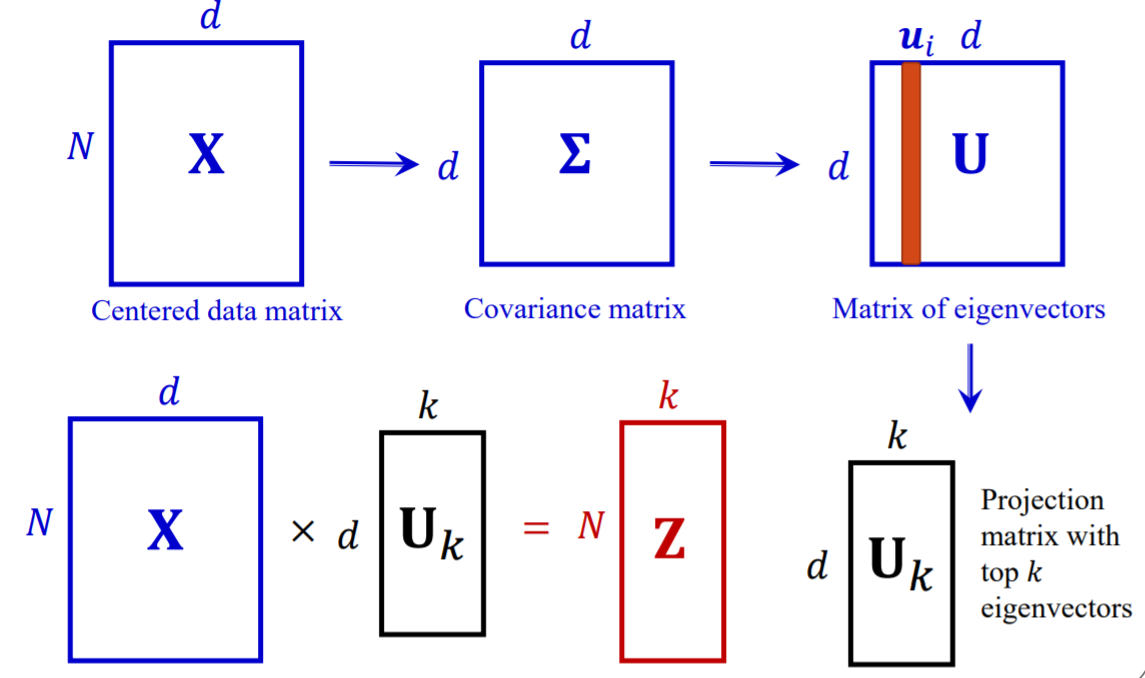
\includegraphics[width=\linewidth]{fig/pca1.PNG}
\subsection*{Computing Eigenvalues/ Eigenvectors}
With the covariance matrix:
\[\tilde{\Sigma} = \frac{1}{N-1}X^TX\]

Define a d-by-d square matrix A, such that
\[A = X^TX\]
Obtain eigenvectors and eigenvalues for A by performing SVD on X\\
As A is positive semidefinite, all eigenvalues are non-negative

\subsection*{Singular Value Decomposition (SVD)}
The SVD of X (N-by-d) has the following form:
\[X = VDU^T\]
Therefore,
\[A = X^TX = (VDU^T)^TVDU^T\]
\[A = UD^TV^TVDU^T\]
$V^TV = I$,
\[A = UD^TDU^T\]
Denoting $\bar{D} = D^T D$,
\[A = U\bar{D}U^T\]
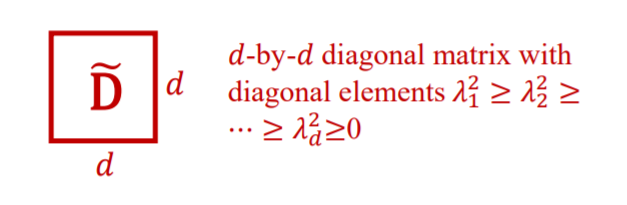
\includegraphics[width=\linewidth]{fig/pca2.PNG}
$U^TU = I$,
\[AU = U\bar{D}, \text{or }AU = \bar{D}U\]
Therefore, each column of U is an eigenvector of A, $\bar{D}$
is the square matrix where the diagonal values correspond to the eigenvalues.

\section{Others}
\[\text{Precision} = \frac{\text{TP}}{\text{TP}+\text{FP}}\]

Precision is a metric that quantifies the number of correct positive predictions made.\\\\
Precision, therefore, calculates the \textbf{accuracy for the minority class}.\\\\
It is calculated as the ratio of correctly predicted positive examples divided by the total number of positive examples that were predicted.

\[\text{Recall} = \frac{\text{TP}}{\text{TP}+\text{FN}}\]

Recall is a metric that quantifies the number of correct positive predictions made out of all positive predictions that could have been made.\\\\
Unlike precision that only comments on the correct positive predictions out of all positive predictions, recall provides an indication of missed positive predictions.\\\\
In this way, recall provides some notion of the \textbf{coverage of the positive class}.

% \input{sections/mengen}
% \input{sections/relationen}
% \input{sections/abbildungen}
% \input{sections/beweise} 
% \input{sections/graphen}
% \input{sections/graphalgo}
% \input{sections/bool}
% \input{sections/formeln}
\end{multicols*}
\end{document}